
The general equation of a circle can be expressed as:
\begin{align}
\vec{x^T}\vec{x} + 2\vec{u^T}\vec{x} + f = 0 \label{rams/4/2/16/eq:4}
\end{align}
If $r$ is radius and $\vec{c}$ is the centre of the circle we have:
\begin{align}
f &=\vec{u}^T\vec{u}-r^2  \label{rams/4/2/16/eq:5} \\  
\vec{c} &=-\vec{u}
\end{align}

The general equation of a second degree can be expressed as :
\begin{align}
\vec{x}^T\vec{V}\vec{x}+2\vec{u}^T\vec{x}+f=0\label{rams/4/2/16/eq:6}
\end{align}
The points of contact $\vec{q}$, of a line with a normal vector $\vec{n}$ to the conics in \eqref{rams/4/2/16/eq:6} are given by:
\begin{align}
\vec{q} = \vec{V}^{-1}\brak{\kappa \vec{n}-\vec{u}} \label{rams/4/2/16/eq:7} \\
\kappa = \pm \sqrt{\frac{\vec{u}^T\vec{V}^{-1}\vec{u}-f}{\vec{n}^T\vec{V}^{-1}\vec{n}}}\label{rams/4/2/16/eq:8}
\end{align}
We know that, for a circle, 
\begin{align}
\vec{V} = \vec{I}\label{rams/4/2/16/eq:9}  
\end{align}
and from the properties of an Identity matrix, 
\begin{align}
\vec{I}^{-1} &= \vec{I} \\
\vec{I}\vec{X} &= \vec{X}   
\end{align}

The touch points of the circles of the form \eqref{rams/4/2/16/eq:4}  with line \eqref{rams/4/2/16/eq:1} are determined by:
\begin{align}
\kappa_{1} &= \pm \sqrt{\frac{\vec{u}^T\vec{u}-f}{\myvec{0 & 1 }\myvec{0 \\ 1 }}} \\
\kappa_{1} &= \pm \sqrt{\frac{r^2}{\myvec{0 & 1 }\myvec{0 \\ 1 }}} \\
& =  \pm {r}
\end{align}
Therefore we have:
\begin{align}
\vec{q_{1}} &= \pm{r}\myvec{0 \\ 1} - \vec{u}
\end{align}
Now $\vec{q_{1}}$ lies on the line \eqref{rams/4/2/16/eq:1} therefore,
\begin{align}
\myvec{0 & 1}\Big(\pm{r}\myvec{0 \\ 1} - \vec{u}\Big) &= 0 \\
\implies \myvec{0 & 1}\vec{u} = \pm{r}\label{rams/4/2/16/eq:10}
\end{align}

The touch points of the circles of the form \eqref{rams/4/2/16/eq:4}  with line \eqref{rams/4/2/16/eq:2} are determined by:
\begin{align}
\kappa_{2} &= \pm \sqrt{\frac{\vec{u}^T\vec{u}-f}{\myvec{0 & 1 }\myvec{0 \\ 1 }}} \\
\kappa_{2} &= \pm \sqrt{\frac{r^2}{\myvec{0 & 1 }\myvec{0 \\ 1 }}} \\
& =  \pm {r}
\end{align}
Therefore we have:
\begin{align}
\vec{q_{2}} &= \pm{r}\myvec{0 \\ 1} - \vec{u}
\end{align}
Now $\vec{q_{2}}$ lies on the line \eqref{rams/4/2/16/eq:2} therefore,
\begin{align}
\myvec{0 & 1}\Big(\pm{r}\myvec{0 \\ 1} - \vec{u}\Big) &= 4 \\
\implies \myvec{0 & 1}\vec{u} = \pm{r}-4\label{rams/4/2/16/eq:11}
\end{align}

The touch points of the circles of the form \eqref{rams/4/2/16/eq:4}  with line \eqref{rams/4/2/16/eq:3} are determined by:
\begin{align}
\kappa_{3} &= \pm \sqrt{\frac{\vec{u}^T\vec{u}-f}{\myvec{2 & 1 }\myvec{2 \\ 1 }}} \\
\kappa_{3} &= \pm \sqrt{\frac{r^2}{\myvec{2 & 1 }\myvec{2 \\ 1 }}} \\
& =  \pm \dfrac{r}{\sqrt{5}}
\end{align}
Therefore we have:
\begin{align}
\vec{q_{3}} &= \pm \dfrac{r}{\sqrt{5}}\myvec{2 \\ 1} - \vec{u}
\end{align}
Now $\vec{q_{3}}$ lies on the line \eqref{rams/4/2/16/eq:3} therefore,
\begin{align}
\myvec{2 & 1}\Big(\pm \dfrac{r}{\sqrt{5}}\myvec{2 \\ 1} - \vec{u}\Big) &= 2 \\
\implies \myvec{2 & 1}\vec{u} = \pm\sqrt{5}r-2\label{rams/4/2/16/eq:12}
\end{align}

Now we need to solve the equations \eqref{rams/4/2/16/eq:10}, \eqref{rams/4/2/16/eq:11} and \eqref{rams/4/2/16/eq:12} written below to obtain $\vec{u}$ and $r$ :
\begin{align}
\myvec{0 & 1}\vec{u} &= \pm{r}\nonumber\\
\myvec{0 & 1}\vec{u} &= \pm{r}-4\nonumber\\
\myvec{2 & 1}\vec{u} &= \pm\sqrt{5}r-2\nonumber
\end{align}
The first two equations are consistent and give a positive solution for $r$ only when they are of the form :
\begin{align}
\myvec{0 & 1}\vec{u} &= -r\nonumber\\
\myvec{0 & 1}\vec{u} &= r-4\nonumber
\end{align}
which upon solving give :
\begin{align}
r &= 2\label{rams/4/2/16/eq:13}\\
\myvec{0 & 1}\vec{u} &= -2\label{rams/4/2/16/eq:14}
\end{align}
Now putting $r=2$ in the third equation we have:
\begin{align}
\myvec{2 & 1}\vec{u} &= \pm2\sqrt{5}-2\label{rams/4/2/16/eq:15}
\end{align}
Let us say $\vec{u} = \myvec{\alpha \\ \beta}$. Substituting $\vec{u}$ in \eqref{rams/4/2/16/eq:14} we have:
\begin{align}
\myvec{0 & 1}\myvec{\alpha \\ \beta} &= -2\\
\implies \beta = -2
\end{align}
Substituting $\vec{u}$ in \eqref{rams/4/2/16/eq:15} we have:
\begin{align}
\myvec{2 & 1}\myvec{\alpha \\ \beta} &= \pm2\sqrt{5} -2\\
\myvec{2 & 1}\myvec{\alpha \\ -2} &= \pm2\sqrt{5} -2\\
\implies \alpha &= \pm\sqrt{5}
\end{align}
Therefore we have:
\begin{align}
\vec{u} = \myvec{\pm\sqrt{5} \\ -2}
\end{align}
Hence the value of $f$ is given by:
\begin{align}
f &=\vec{u}^T\vec{u}-r^2\\
f &= \myvec{\pm\sqrt{5} & -2}\myvec{\pm\sqrt{5} \\ -2} - 2^2\\
f &= 5
\end{align}
Hence the tangent circles are given by the equations:
\begin{align}
\vec{x^T}\vec{x} + \myvec{2\sqrt{5} & -4}\vec{x} + 5 &= 0 \\
\vec{x^T}\vec{x} + \myvec{-2\sqrt{5} & -4}\vec{x} + 5 &= 0
\end{align}
The illustration of the circles and the lines is shown in Fig.     \ref{rams/4/2/16/Tangent circles to 3 given lines}
\begin{figure}[!ht]
       \centering
    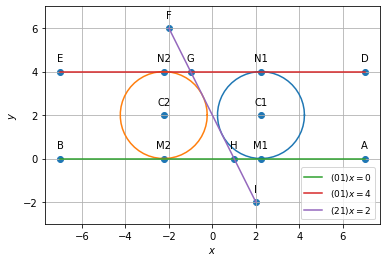
\includegraphics[width=\columnwidth] {solutions/4/2/16/Assignment_3_Fig_1.png}
    \caption{Circles touching given lines with centres C1,C2}
    \label{rams/4/2/16/Tangent circles to 3 given lines}
\end{figure}


